\documentclass[a4paper,12pt]{report}
\usepackage[utf8]{inputenc}
\usepackage{graphicx}
\usepackage[catalan]{babel}
\usepackage[backend=bibtex,sorting=none]{biblatex}
\addbibresource{references.bib}
\usepackage[headheight=35pt]{geometry}
\usepackage[bottom]{footmisc}
\usepackage{float}

\usepackage{fancyhdr}
\pagestyle{fancy}
\fancyhead{}
\fancyhead[RO,RE]{\leftmark}
\fancyhead[LO,LE]{
\includegraphics[width=0.3\textwidth]{images/fib-upc-logo}}
\fancyfoot{}
\fancyfoot[CO,CE]{\thepage}

\usepackage{titlesec}
\titleformat{\chapter}[hang] 
{\normalfont\huge\bfseries}{\thechapter.}{1em}{} 

\usepackage{array}
\usepackage{bookmark}
\usepackage[toc,page]{appendix}
\usepackage{rotating}
\usepackage[gen]{eurosym}
\DeclareUnicodeCharacter{20AC}{\euro{}}
\usepackage[table]{xcolor}
\usepackage{hyperref}

\renewcommand\appendixtocname{Apèndix}
\renewcommand\appendixpagename{Apèndix}

\begin{document}

	\newgeometry{bottom=2.5cm}

	\begin{titlepage}
		\begin{center}
			\vspace*{1cm}

			\line(1,0){400}\\
			%\noindent\hrulefill\\
			\vspace{0.3cm}
			\Huge
			\textbf{Sistema d'autolocalització per a robots mòbils mitjançant tècniques de visió per computador}\\
			%\noindent\hrulefill
			\line(1,0){400}

			\vspace{1.0cm}
			\Large
			Joan Rodas Cusidó\\
			02-10-2016

			\vfill
			\LARGE
			\textit{Treball final de grau en eng. informàtica\\
			Tecnologies de la informació}\\
			\vspace{0.3cm}
			\normalsize{Lliurable 2 - GEP}

			\vspace{1.6cm}

			
\includegraphics[width=0.2\textwidth]{images/logo}
			%
\includegraphics[width=0.7\textwidth]{images/fib-upc-logo}
			
			%\vspace{1cm}
			\vspace{0.5cm}

			\Large
			Facultat d'Informàtica de Barcelona\\
			Universitat Politècnica de Catalunya\\
			%\vspace{0.5cm}
			Director: Joan Climent Vilaró
		\end{center}
	\end{titlepage}
	
	
	\restoregeometry
	\newgeometry{bottom=4.5cm}
	\setcounter{page}{2}
	
	\tableofcontents
	\chapter{Introducció}
	\textit{Aquest projecte es desenvolupa com a treball final de grau dels estudis de grau en enginyeria informàtica, de l'especialitat en tecnologies de la informació.
Es tracta d'un projecte de modalitat A, realitzat a la Facultat d'Informàtica de Barcelona (Universitat Politècnica de Catalunya) i proposat pel director Joan Climent,
del departament d'ESAII (Enginyeria de Sistemes, Automàtica i Informàtica Industrial).}\\\\\\\\
Els avenços tecnològics dels últims anys, han millorat la capacitat de les màquines per extreure informació i resoldre problemes de manera autònoma, imitant cada vegada millor
el comportament humà. En aquest treball, es treballarà la visió per computador aplicada a un problema de robòtica.\\\\
El projecte es divideix en 10 capítols. El primer capítol serveix com a introducció del projecte, on s'explica l'abast, objectiu, motivació i estat de l'art de les tecnologies a tractar.
En el segon capítol es detallen els recursos utilitzats per realitzar el treball.\\\\
Els capítols 3 a 7 conformen el treball principal. Al tercer capítol s'explica el disseny i l'aquitectura del sistema desenvolupat. Al cuart, l'estructura i configuració del servidor. Les tecniques de visió
utilitzades s'expliquen al cinqué capítol, amb la seva implementació detallada al sisé. Al capítol 7 s'explicaran els experiments realitzats i els resultats obtinguts.\\\\
Al capítol 8 podeu trobar un anàlisi de la gestió econòmica del projecte, on es detallen els costos humans, de programari, de maquinari, indirectes i possibles imprevistos. I al nové capítol
es presenta l'informe de sostenibilitat. Per acabar, hi haurà les conclusions del projecte, on es valorarà l'aportació del projecte a nivell personal i si s'han complert els objectius inicials proposats.

%\section{Context}
%	Aquest projecte es desenvolupa com a treball final de grau dels estudis de grau en enginyeria informàtica, de l'especialitat en tecnologies de la informació.
%	Es tracta d'un projecte de modalitat A, realitzat a la Facultat d'Informàtica de Barcelona (Universitat Politècnica de Catalunya) i proposat pel director Joan Climent,
%	del departament d'ESAII (Enginyeria de Sistemes, Automàtica i Informàtica Industrial).
\section{Descripció del problema}
	El treball pretén resoldre un problema d'autolocalització de robots mòbils en un entorn variable, de tal manera que el robot sigui capaç de desplaçar-se d'un punt inicial a un punt final escollit per
	l'usuari. Per fer això, s'utilitzaran diverses tècniques de visió per ordinador.
\section{Motivació}
	Visió per computador i Robòtica van ser sense cap mena de dubte dos de les assignatures més interessants que he cursat a la universitat, així que quan vaig veure la oferta del projecte vaig pensar que
	seria una bona idea per profunditzar els meus coneixements sobre la materia.
\section{Actors implicats}
	En aquesta secció es descriuen els actors implicats del projecte, és a dir, totes aquelles persones que es veuran beneficiades directa o indirectament amb la realització d'aquest.\\
	\begin{itemize}
		\item \textbf{Autor/Desenvolupador:} És el màxim responsable del projecte. En tractar-se d'un treball final de grau, l'autor del projecte serà també el màxim beneficiari, ja que la realització d'aquest li permetrà acabar la carrera d'enginyeria informàtica.
		\item \textbf{Usuaris:} Qualsevol persona qui ho desitgi, tindrà accés a tots els codis desenvolupats durant el projecte, ja que es llançaran sota una llicència de programari lliure que permetrà veure i adaptar el codi a les necessitats d'altres usuaris.
		\item \textbf{Altres beneficiaris:} Qualsevol persona, empresa o institució interessada podrà utilitzar el sistema desenvolupat i adaptar-lo a les seves necessitats, com podria ser per exemple un sistema de transport d'equipatge basat en robots.
	\end{itemize}
\newpage
\section{Estat de l'art}
	\subsection{Visió per computador}
		La visió per computador\cite{Szeliski} és una ciència que té com a objectiu dotar les màquines o ordinadors de la capacitat de ``veure''.
		Es basa en l'extracció i anàlisi de dades obtingudes a partir d'imatges.\\\\
		Algunes de les aplicacions de la visió per computador són:\\
		\begin{itemize}
			\item Vehicles autònoms
			\item Realitat augmentada
			\item Reconeixement facial
			\item Restauració d'imatges
			\item Inspecció industrial 
			\item Robòtica\\
		\end{itemize}
		En aquest treball, ens interessa utilitzar la visió per computador en el camp de la robòtica, per aconseguir guiar a un robot mòbil cap a un objectiu
		determinat basant-se en la detecció d'un punt o regió en una imatge.
		\subsubsection{Nous algorismes}
			En els darrers anys, han aparegut nous algorismes d'obtenció de punts i extracció de característiques que suposen una alternativa als clàssics SIFT\cite{SIFT}
			( Scale Invariant Feature Transform) i SURF\cite{SURF} (Speeded-Up Robust Features). Alguns d'aquests algorismes són BinBoost\cite{Trzcinski13a} o un dels més recents:
			LATCH\cite{LeviHassner2016LATCH}\\\\
			En aquest projecte s'analitzarà si es adequat emprar algun d'aquests algorismes en la implementació del sistema d'autolocalització. 
\newpage
	\subsection{Robòtica}
		La robòtica és un camp de la tecnologia que estudia el disseny i la construcció de robots.\\\\
		Que és, doncs, un robot? Al llarg de la historia, s'han donat diverses definicions del concepte de robot, sense existir encara una definició exacta acceptada per tothom. I a mesura que passa el temps,
		cada vegada resulta més complicat determinar si una màquina és o no un robot. Per no complicar-nos massa, entendrem com a robot una màquina programable capaç de realitzar una sèrie de
		tasques concretes interactuant amb l'entorn, ja sigui de manera automàtica o dirigida.\\\\
		Existeixen diversos tipus de robots, podent fer una classificació senzilla segons la seva arquitectura: robots mòbils, poliarticulats (industrials, mèdics, etc.), humanoides, 
		zoomòrfics\footnote{\textbf{Robots zoomòrfics:} Robots que imiten característiques pròpies de determinats animals.} i híbrids.\\\\
		Els robots mòbils, que són els que ens interessen per aquest projecte, acostumen a tenir una sèrie de sensors i dispositius per permetre'n el desplaçament, la localització, esquivar obstacles i
		realitzar tasques concretes. Alguns exemples de sensors utilitzats per robots mòbils són:\\
		\begin{itemize}
			\item Odometria: S'utilitza la informació obtinguda amb sensors de moviment (\textit{encoders} a les rodes, per exemple) per estimar la posició del robot respecte a la inicial.
			\item GPS (Global Positioning System): Es determina la ubicació del robot amb la xarxa de satèl·lits.
			\item Sensors de contacte: Permeten detectar si el robot està en contacte amb un altre objecte.
			\item Sensors d'ultrasons: Detecten objectes mitjançant ones ultrasòniques.
			\item Acceleròmetre: Determina l'acceleració del robot quan es mou. 
			\item Càmera: Permet capturar imatges de l'entorn.\\
		\end{itemize}
		En el nostre cas, només ens interessaran les dades obtingudes a través d'una càmera, és a dir, les imatges. El treball no se centrarà per tant en la part robòtica del sistema, i no es tindran en compte
		els sensors i algorismes necessaris per poder moure el robot.\\\\
		En cas d'aplicar el sistema desenvolupat en robots en un futur, aleshores s'hauran de tenir en compte altres sensors per permetre el moviment
		de la màquina i arribar a la destinació evitant obstacles.
\section{Objectius}
	L'objectiu principal del projecte consisteix a dissenyar i desenvolupar un sistema d'autolocalització per a robots mòbils.\\\\
	Aquest sistema estarà basat en tècniques de visió per computador i consistirà, bàsicament, a comparar dues imatges (una global i una altra capturada pel robot)
	i localitzar un punt o regió seleccionat per l'usuari.\\\\	
	Per arribar a aquest objectiu, es dividirà el treball en diverses fases:\\
	\begin{itemize}
		\item Estudi dels diferents algorismes de visió existents
		\item Obtenció de \textit{keypoints} en una imatge
		\item Extracció de característiques
		\item \textit{Matching} de dues imatges
	\end{itemize}
\section{Requeriments}
	El sistema d'autolocalització implementat ha de complir amb una sèrie de requeriments mínims presentats a continuació:\\
	\begin{itemize}
		\item L'usuari ha de poder seleccionar un punt o regió d'interès en una imatge donada.
		\item El sistema ha de ser capaç d'adaptar-se mínimament a diverses condicions de l'entorn (canvis de lluminositat, perspectiva, etc.).
	\end{itemize}
\newpage
\section{Obstacles}
	Durant la planificació i realització del treball, s'hauran de tenir en compte els possibles obstacles que es trobaran. A continuació es detallen alguns dels problemes que es podran trobar.
	\subsubsection{Noves eines}
		Un dels principals obstacles serà el fet de treballar amb noves eines i algorismes. Per tal d'evitar problemes en aquest aspecte, caldrà fer una planificació acurada i documentar-se apropiadament.
		També serà important mantenir una bona comunicació amb el tutor en tot moment, per poder resoldre possibles dubtes referents als algorismes.
	\subsubsection{Calendari}
		Un altre obstacle important serà la falta de temps, ja que està previst realitzar el projecte en el transcurs d'un quadrimestre. Gestionar correctament el temps serà clau per aconseguir
		finalitzar el projecte sense problemes. Per tant, s'haurà de fer una planificació el més realista possible i escollir una metodologia de treball adequada i flexible.
	\subsubsection{Errors de programació}
		Com a qualsevol projecte on s'ha de programar, el codi serà una font important d'errors. Per això, caldrà realitzar diverses proves cada vegada que es realitzi una modificació en el codi
		o s'implementi una nova funcionalitat.
	\subsubsection{Condicions variables en les imatges}
		Les imatges capturades a través d'una càmera no presentaran sempre les mateixes condicions. La lluminositat, perspectiva o resolució de la imatge 
		influiran a l'hora de processar les imatges i comparar-les.\\\\
		Per intentar minimitzar aquests efectes, s'analitzaran diversos algorismes d'obtenció de punts i extracció de característiques. 
		També s'estudiarà si és necessari realitzar un preprocessament o filtratge de les imatges abans d'aplicar els algorismes.
\newpage
\section{Ampliacions}
	Encara que el calendari és força estricte i no hi ha gaire marge d'ampliació, es podria estendre el projecte amb les següents ampliacions:\\
	\begin{itemize}
		\item Anàlisi del rendiment d'algorismes alternatius per l'obtenció de punts i característiques de les imatges.
		\item Creació d'una aplicació d'Android que permeti seleccionar un punt o regió d'una imatge.
		\item Execució del codi del sistema via servidor web, utilitzant les dades enviades per l'aplicació d'Android.
	\end{itemize}
\section{Metodologia}
	Per aquest projecte, s'utilitzarà una metodologia de treball àgil amb cicles de desenvolupament curts.
	Com que només hi ha un desenvolupador, no s'utilitzaran exactament les metodologies Scrum o XP\cite{Pxp} (Extreme Programming),
	però sí que s'aplicaran moltes de les pràctiques pròpies d'aquestes dues metodologies (proves, simplicitat, refacció de codi, etc.).
	Això ens donarà més flexibilitat a l'hora de fer canvis i adaptar-nos a una nova planificació.\\\\
	Es començarà treballant amb imatges de prova (casos senzills) i algorismes coneguts com ara Harris\cite{Harris} i SIFT. Més endavant, s'aniran introduint modificacions en el codi per intentar aconseguir un
	sistema capaç de funcionar amb fotografies ``reals'' i es provaran altres algorismes de visió per computador.\\\\
	Per altra banda, s'utilitzarà el mètode en cascada per la realització del curs de GEP.
\section{Eines de desenvolupament}
	El codi del projecte es desenvoluparà amb python i s'utilitzaran, sempre que sigui possible, eines de programari lliure o de codi obert.\\\\
	En cas de crear una aplicació per a dispositius Android, es realitzarà mitjançant Android Studio (Java).
	\subsection{OpenCV}
		Per tal d'utilitzar algorismes de visió per computador en el codi amb relativa facilitat, s'utilitzarà la biblioteca de codi obert OpenCV\cite{OpenCV} (Open Source Computer Vision Library),
		disponible per a python. La versió emprada serà la 3.1.\\\\
		En concret, hi haurà tres passos indispensables que faran ús d'aquesta biblioteca:\\
		\begin{itemize}
			\item {Obtenció de punts en una imatge}
			\item {Extracció de característiques}
			\item \textit{Matching} de dues imatges
		\end{itemize}
\section{Eines de seguiment}
	A continuació es detallen les eines de programari usades per fer el seguiment del treball final de grau:
	\subsubsection{LibreOffice Calc}
		Per fer un seguiment de les hores dedicades al projecte, es crearà un full de càlcul amb les hores diàries dedicades a cada tasca. S'utilitzarà LibreOffice Calc, inclòs en
		la \textit{suite} ofimàtica LibreOffice.
	\subsubsection{Gantt Project}
		Per tal d'organitzar totes les tasques a realitzar i mirar si hi ha desviacions respecte el pla inicial, s'utilitzarà l'eina de \textit{software} lliure 
		Gantt Project\cite{GanttProject}. Aquesta eina ens permetrà realitzar tant un diagrama de Gantt com un diagrama de PERT.
	\subsubsection{Git + Github}
		Tot i que no es tracta d'un projecte col·laboratiu (només hi ha un desenvolupador), s'ha decidit utilitzar el sistema de control de versions Git juntament amb la pàgina web Github. 
		D'aquesta manera es facilitarà treballar amb diverses màquines i portar un control dels canvis realitzats. A més, permetrà compartir el codi amb el director amb facilitat.
	\section{Mètode de validació}
		Es faran validacions parcials durant la realització del projecte, fent proves del sistema amb diverses imatges.
	\subsubsection{Contacte amb el director}
		Hi haurà reunions presencials amb el director, així com comunicació via correu electrònic, per tal de resoldre dubtes i validar la feina realitzada. També es realitzarà una reunió de seguiment abans
		del 19 de decembre, per conèixer l'estat del projecte i poder escollir el torn de lectura.


	\chapter{Definició de l'abast}
	\section{Objectius}
	L'objectiu principal del projecte consisteix a dissenyar i desenvolupar un sistema d'autolocalització per a robots mòbils.\\\\
	Aquest sistema estarà basat en tècniques de visió per computador i consistirà, bàsicament, a comparar dues imatges (una global i una altra capturada pel robot)
	i localitzar un punt o regió seleccionat per l'usuari.\\\\	
	Per arribar a aquest objectiu, es dividirà el treball en diverses fases:\\
	\begin{itemize}
		\item Estudi dels diferents algorismes de visió existents
		\item Obtenció de \textit{keypoints} en una imatge
		\item Extracció de característiques
		\item \textit{Matching} de dues imatges
	\end{itemize}
\section{Requeriments}
	El sistema d'autolocalització implementat ha de complir amb una sèrie de requeriments mínims presentats a continuació:\\
	\begin{itemize}
		\item L'usuari ha de poder seleccionar un punt o regió d'interès en una imatge donada.
		\item El sistema ha de ser capaç d'adaptar-se mínimament a diverses condicions de l'entorn (canvis de lluminositat, perspectiva, etc.).
	\end{itemize}
\section{Obstacles}
	Durant la planificació i realització del treball, s'hauran de tenir en compte els possibles obstacles que es trobaran. A continuació es detallen alguns dels problemes que es podran trobar.
	\subsection{Noves eines}
		Un dels principals obstacles serà el fet de treballar amb noves eines i algorismes. Per tal d'evitar problemes en aquest aspecte, caldrà fer una planificació acurada i documentar-se apropiadament.
		També serà important mantenir una bona comunicació amb el tutor en tot moment, per poder resoldre possibles dubtes referents als algorismes.
	\subsection{Calendari}
		Un altre obstacle important serà la falta de temps, ja que està previst realitzar el projecte en el transcurs d'un quadrimestre. Gestionar correctament el temps serà clau per aconseguir
		finalitzar el projecte sense problemes. Per tant, s'haurà de fer una planificació el més realista possible i escollir una metodologia de treball adequada i flexible.
	\subsection{Errors de programació}
		Com a qualsevol projecte on s'ha de programar, el codi serà una font important d'errors. Per això, caldrà realitzar diverses proves cada vegada que es realitzi una modificació en el codi
		o s'implementi una nova funcionalitat.
	\subsection{Condicions variables en les imatges}
		Les imatges capturades a través d'una càmera no presentaran sempre les mateixes condicions. La lluminositat, perspectiva o resolució de la imatge 
		influiran a l'hora de processar les imatges i comparar-les.\\\\
		Per intentar minimitzar aquests efectes, s'analitzaran diversos algorismes d'obtenció de punts i extracció de característiques. 
		També s'estudiarà si és necessari realitzar un preprocessament o filtratge de les imatges abans d'aplicar els algorismes.
\section{Ampliacions}
	Encara que el calendari és força estricte i no hi ha gaire marge d'ampliació, es podria estendre el projecte amb les següents ampliacions:\\
	\begin{itemize}
		\item Anàlisi del rendiment d'algorismes alternatius per l'obtenció de punts i característiques de les imatges.
		\item Creació d'una aplicació d'Android que permeti seleccionar un punt o regió d'una imatge.
		\item Execució del codi del sistema via servidor web, utilitzant les dades enviades per l'aplicació d'Android.
	\end{itemize}
\section{Metodologia}
	Per aquest projecte, s'utilitzarà una metodologia de treball àgil amb cicles de desenvolupament curts.
	Com que només hi ha un desenvolupador, no s'utilitzaran exactament les metodologies Scrum o XP\cite{Pxp} (Extreme Programming),
	però sí que s'aplicaran moltes de les pràctiques pròpies d'aquestes dues metodologies (proves, simplicitat, refacció de codi, etc.).
	Això ens donarà més flexibilitat a l'hora de fer canvis i adaptar-nos a una nova planificació.\\\\
	Es començarà treballant amb imatges de prova (casos senzills) i algorismes coneguts com ara Harris\cite{Harris} i SIFT. Més endavant, s'aniran introduint modificacions en el codi per intentar aconseguir un
	sistema capaç de funcionar amb fotografies ``reals'' i es provaran altres algorismes de visió per computador.\\\\
	Per altra banda, s'utilitzarà el mètode en cascada per la realització del curs de GEP.
\section{Eines de desenvolupament}
	El codi del projecte es desenvoluparà amb python i s'utilitzaran, sempre que sigui possible, eines de programari lliure o de codi obert.\\\\
	En cas de crear una aplicació per a dispositius Android, es realitzarà mitjançant Android Studio (Java).
	\subsection{OpenCV}
		Per tal d'utilitzar algorismes de visió per computador en el codi amb relativa facilitat, s'utilitzarà la biblioteca de codi obert OpenCV\cite{OpenCV} (Open Source Computer Vision Library),
		disponible per a python. La versió emprada serà la 3.1.\\\\
		En concret, hi haurà tres passos indispensables que faran ús d'aquesta biblioteca:\\
		\begin{itemize}
			\item {Obtenció de punts en una imatge}
			\item {Extracció de característiques}
			\item \textit{Matching} de dues imatges
		\end{itemize}
\section{Eines de seguiment}
	A continuació es detallen les eines de programari usades per fer el seguiment del treball final de grau:
	\subsection{LibreOffice Calc}
		Per fer un seguiment de les hores dedicades al projecte, es crearà un full de càlcul amb les hores diàries dedicades a cada tasca. S'utilitzarà LibreOffice Calc, inclòs en
		la \textit{suite} ofimàtica LibreOffice.
	\subsection{Gantt Project}
		Per tal d'organitzar totes les tasques a realitzar i mirar si hi ha desviacions respecte el pla inicial, s'utilitzarà l'eina de \textit{software} lliure 
		Gantt Project\cite{GanttProject}. Aquesta eina ens permetrà realitzar tant un diagrama de Gantt com un diagrama de PERT.
	\subsection{Git + Github}
		Tot i que no es tracta d'un projecte col·laboratiu (només hi ha un desenvolupador), s'ha decidit utilitzar el sistema de control de versions Git juntament amb la pàgina web Github. 
		D'aquesta manera es facilitarà treballar amb diverses màquines i portar un control dels canvis realitzats. A més, permetrà compartir el codi amb el director amb facilitat.
	\section{Mètode de validació}
		Es faran validacions parcials durant la realització del projecte, fent proves del sistema amb diverses imatges.
	\subsubsection{Contacte amb el director}
		Hi haurà reunions presencials amb el director, així com comunicació via correu electrònic, per tal de resoldre dubtes i validar la feina realitzada.

	\chapter{Planificació}
	%\newcommand*{\thead}[1]{\multicolumn{1}{|l|}{\bfseries #1}}
\def\arraystretch{1.4}
\definecolor{tableHeader}{RGB}{211, 127, 47}
\definecolor{myOrange}{RGB}{255, 230, 210}
\newcolumntype{x}[1]{>{\centering\arraybackslash\hspace{0pt}}m{#1}}

\section{Planificació temporal}
	\label{sec:planificacio}
	Inicialment s'esperava realitzar el treball entre els mesos de setembre i gener, però finalment s'ha optat per ampliar el termini fins a l'abril. La càrrega total serà d'unes 480 hores.
	%La dedicació setmanal estimada serà d'unes 20 hores.
	\\\\
	Es dividirà el projecte en quatre blocs, descrits a continuació:\\

	\begin{table}[H]
		\begin{center}
			\rowcolors{2}{myOrange}{}
			\begin{tabular}{p{1.5cm} !{\vrule width -1pt}p{6cm} !{\vrule width -1pt}l !{\vrule width -1pt}l}
				\rowcolor{tableHeader}
				\textbf{Bloc} & \textbf{Descripció} & \textbf{Metodologia} & \textbf{Hores} \\ %\hline
				Bloc 0 & Preparació de l'entorn & - & 5h \\
				Bloc 1 & Curs de GEP & Cascada & 75h \\
				Bloc 2 & Desenvolupament del projecte & Àgil & 355h \\
				Bloc 3 & Preparació de la defensa & - & 45h \\
			\end{tabular}
		\end{center}
		\caption{Blocs del projecte}
	\end{table}

	\subsection{Bloc 0: Preparació de l'entorn}
		Inicialment, s'instal·larà tot el programari necessari per començar a desenvolupar el projecte i es faran algunes proves bàsiques per familiaritzar-se amb el nou entorn de treball.
		Aquest primer bloc tindrà una durada aproximada de 5 hores.\\\\
		Per poder començar a treballar en el projecte, caldrà instal·lar:\\
		\begin{itemize}
			\item \textbf{Desenvolupament:} Python, OpenCV, Geany i Git.
			\item \textbf{Curs de GEP:} Gantt Project.
			\item \textbf{Documentació:} {\LaTeX} i Zathura.
		\end{itemize}

	\subsection{Bloc 1: Curs de GEP}
		Aquest bloc correspon a la realització del curs de GEP, amb inici el dia 19/09/2016 i finalització el 24/10/2016 (amb una presentació final entre el 7 i l'11 de novembre).
		Té com a dependència el bloc 0.\\\\
		Durant el curs s'entregaran 6 lliurables, detallats a continuació:\\
		\begin{table}[H]
			\begin{center}
				\rowcolors{2}{myOrange}{white}
				\begin{tabular}{p{5cm} !{\vrule width -1pt}x{2.1cm} !{\vrule width -1pt}x{2.4cm} !{\vrule width -1pt}x{1.6cm} !{\vrule width -1pt}x{1.6cm}}
					\rowcolor{tableHeader}
					\textbf{Descripció} & \textbf{Inici} & \textbf{Finalització} & \textbf{Durada} & \textbf{Hores} \\ %\hline
					Introducció i abast & 19/09/2016 & 27/09/2016 & 9 dies & 16h \\
					Planificació temporal & 28/09/2016 & 03/10/2016 & 6 dies & 9h \\
					Gestió econòmica i sostenibilitat & 04/10/2016 & 10/10/2016 & 7 dies & 10h \\
					Presentació en vídeo & 11/10/2016 & 17/10/2016 & 7 dies & 11h \\
					Plec de condicions & 18/10/2016 & 24/10/2016 & 7 dies & 13h \\
				Document final + presentació & 18/10/2016 & 24/10/2016 & 7 dies & 16h
				\end{tabular}
			\end{center}
			\caption{Lliurables de GEP}
		\end{table}

	\subsection{Bloc 2: Desenvolupament del projecte}
			El bloc principal consistirà en el desenvolupament del projecte en si mateix: buscar informació, implementar el codi, redactar la memòria, etc.\\\\
			Aquest bloc té com a dependència el bloc 0 i es dividirà en quatre tasques.\\
			\begin{table}[H]
				\begin{center}
					\rowcolors{2}{myOrange}{white}
					\begin{tabular}{p{5cm} !{\vrule width -1pt}x{2.1cm} !{\vrule width -1pt}x{2.4cm} !{\vrule width -1pt}x{1.6cm} !{\vrule width -1pt}x{1.6cm}}
						\rowcolor{tableHeader}
						\textbf{Tasca} & \textbf{Inici} & \textbf{Finalització} & \textbf{Durada} & \textbf{Hores} \\ %\hline
						Implementació i proves & 13/09/2016 & 15/02/2017 & 156 dies & 225h \\
						Experiments & 20/01/2017 & 30/03/2017 & 70 dies & 40h \\
						Ampliacions (opcional) & 01/03/2017 & 30/03/2017 & 30 dies & 40h \\
						Redacció de la memòria & 10/10/2016 & 13/04/2017 & 186 dies & 50h \\
					\end{tabular}
				\end{center}
				\caption{Tasques desenvolupament}
			\end{table}

		\subsubsection{Recerca d'informació, implementació i proves}
			Una part molt important del projecte serà la cerca d'informació i l'estudi de les diverses eines i algorismes a utilitzar (com per exemple OpenCV i les seves funcions).
			Se cercarà informació contínuament i s'aniran fent proves a mesura que s'implementa el codi.\\\\
			La fase d'implementació es dividirà en diverses tasques, que s'aniran realitzant a mesura que avanci el projecte. Algunes d'aquestes tasques seran:
			\begin{itemize}
				\item{Obtenció de keypoints (Harris)}
				\item{Extracció de característiques (SIFT)}
				\item{Matching i homografia}
				\item{Altres algorismes (ORB, BRISK, LATCH...)}
				\item{Disseny de l'aplicació d'Android/web}
				\item{Creació de l'aplicació d'Android/web}
			\end{itemize}
		\subsubsection{Experiments}
			Un cop enllestida la implementació, es procedirà a realitzar diversos experiments amb el programa. Es compararan els resultats obtinguts amb diferents algorismes de visió i es faran
			proves del sistema amb diverses imatges.
		\subsubsection{Ampliacions i millores}
			Un cop realitzats els experiments bàsics, es faran ampliacions i millores en el programa.\\\\
			En cas de patir un retard en la planificació del projecte, s'utilitzarà aquest temps per acabar l'etapa d'experimentació.
		\subsubsection{Redacció de la memòria}
			La memòria s'anirà redactant a mesura que es realitza el projecte. No hi ha per tant cap dependència, encara que es dedicarà més temps en l'etapa final del treball.\\

	\subsection{Bloc 3: Preparació de la defensa}
	En aquest bloc final es revisarà la memòria del projecte i es prepararà la presentació. Està previst dedicar unes 45 hores al bloc, que començarà el dia 28 de març i acabarà el 23 d'abril.
	La defensa del projecte es durà a terme entre els dies 24 i 28 d'abril.

	\subsection{Diagrames}
		Durant la fase de planificació del treball, s'han realitzat diversos diagrames. A continuació podeu trobar els diagrames de PERT i el Gantt del projecte.\\

		\begin{figure}[H]
			\centering
			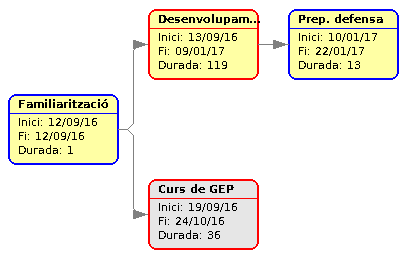
\includegraphics[width=0.7\textwidth]{images/pert-global}
			\caption{PERT del projecte}
		\end{figure}
		\vspace{0.8cm}
		\begin{figure}[H]
			\centering
			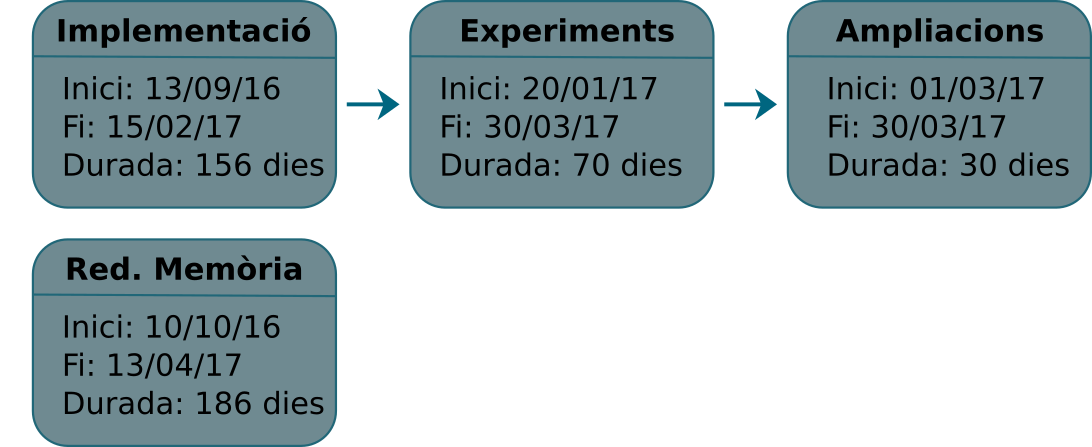
\includegraphics[width=0.7\textwidth]{images/tasques}
			\caption{PERT - tasques desenvolupament}
		\end{figure}

		\restoregeometry
		\newgeometry{bottom=1cm, top=1cm}
		\thispagestyle{empty}
		\begin{sidewaysfigure}
			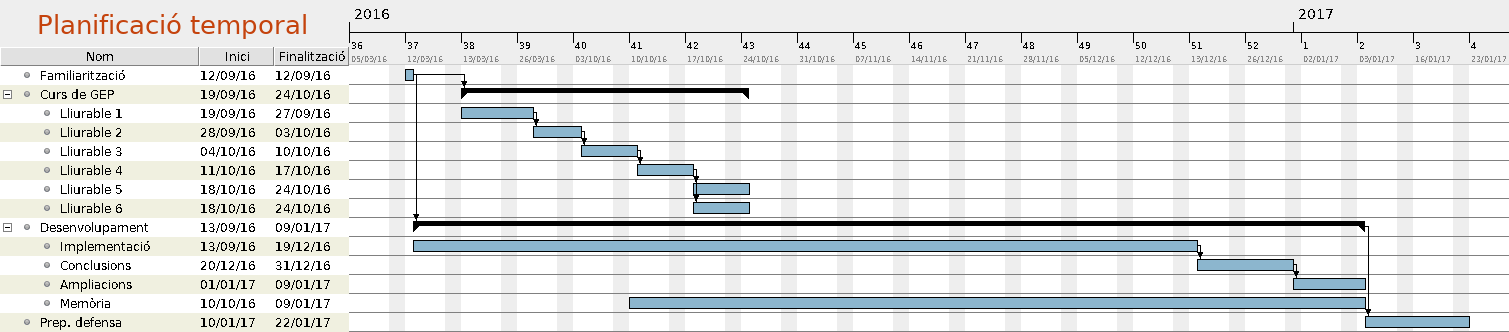
\includegraphics[width=\textheight]{images/gantt}
			\caption{Gantt del projecte}
		\end{sidewaysfigure}
		\restoregeometry
		\newgeometry{bottom=4.5cm}

\section{Recursos}
	En aquesta secció es detallen els recursos necessaris per a la realització del projecte. %A continuació es detallen els recursos humans, de maquinari i de programari utilizats.
	\subsection{Recursos humans}
		El projecte el realitzarà una sola persona, que haurà d'assumir els rols de cap de projecte, analista, dissenyador, programador i \textit{tester}.
		També es comptarà amb l'ajuda del director del projecte, que assumirà el paper de consultor/supervisor.
	\subsection{Recursos de maquinari}
		Per la realització del projecte no serà necessari adquirir cap mena de maquinari específic. Es podrà utilitzar un ordinador personal per treballar a casa i els ordinadors disponibles a la FIB per
		treballar des de la universitat.\\\\
		Es treballarà principalment amb un ordinador equipat amb un processador AMD FX 6300 hexa-core 3.5GHz, 4GB de RAM i 250GB de disc dur SSD. També s'utilitzarà una càmera o \textit{smartphone} qualsevol.\\\\
		Pel servidor s'ha decidit utilitzar una Raspberry Pi 2.
	\subsection{Recursos de programari}
	Durant la realització del projecte i el curs de GEP, s'utilitzaran diverses eines de programari, detallades a continuació:\\
	\begin{table}[H]
		\begin{center}
			\rowcolors{2}{myOrange}{white}
			\begin{tabular}{l !{\vrule width -1pt}p{5cm} !{\vrule width -1pt}p{5cm}}
				\rowcolor{tableHeader}
				\textbf{Nom} & \textbf{Tipus} & \textbf{Ús} \\ %\hline
				Arch Linux/Raspbian & Eina de desenvolupament & Execució del programari \\
				Python & Eina de desenvolupament & Programació \\
				Flask & Eina de desenvolupament & Programació (framework) \\
				OpenCV & Eina de desenvolupament & Algorismes de VC \\
				Nginx & Eina de desenvolupament & Servidor web / proxy \\
				uWSGI & Eina de desenvolupament & Servidor uwsgi \\
				Geany/Atom & Eina de desenvolupament & Programació del codi \\
				Android Studio & Eina de desenvolupament & Programació del codi \\
				Gimp/Inkscape & Eina de desenvolupament & Retocs i creació d'imatges \\
				\LaTeX & Eina de desenvolupament & Redacció de la memòria \\
				Zathura & Eina de desenvolupament & Visualització de pdf \\
				Gantt Project & Eina de gestió & Creació diagrames de Gantt \\
				LibreOffice Calc & Eina de gestió & Control de les hores \\
				Git + GitHub & Desenvolupament i gestió & Control de versions \\
			\end{tabular}
		\end{center}
		\caption{Recursos de programari}
		\label{table:programari}
	\end{table}
	
\section{Desviacions i pla d'actuació}
	\subsubsection{Mala planificació [Impacte: mig]}
		Hi haurà reunions amb el director i s'usaran eines de planificació per mirar de corregir la planificació i acabar el projecte a temps. També es reserven unes hores a l'ampliació del treball,
		que es podrien utilitzar en cas que una tasca s'allargués més del previst. Si fos necessari, es podria incrementar una mica la càrrega de treball setmanal.
	\subsubsection{Fallades de maquinari [Impacte: baix]}
		En cas de fallades en l'ordinador principal, no hi hauria cap problema en utilitzar-ne un altre. No hi ha dependències de hardware i es disposa d'altres ordinadors (a casa i a la FIB).
		Tampoc hi hauria una pèrdua de dades important, ja que es treballa amb GitHub i una còpia local.

	\chapter{Gestió econòmica}
	\def\arraystretch{1.4}
\definecolor{tableHeader}{RGB}{53, 104, 151}
\definecolor{total2}{RGB}{150, 200, 230}
\definecolor{total}{RGB}{240, 240, 240} %GRIS
\definecolor{myGray}{RGB}{236, 242, 248}
\newcolumntype{x}[1]{>{\centering\arraybackslash\hspace{0pt}}m{#1}}

\label{sec:Costos}

%A continuació es detallen els costos necessaris per la realització d'aquest treball.
\section{Recursos de programari}
	Tot el \textit{software} utilitzat en aquest projecte és gratuït i de codi obert. Per tant, el programari no suposarà cap despesa. Podeu trobar el llistat del programari utilitzat
	a la taula \ref{table:programari} (Recursos de programari).

\section{Recursos humans}
	El projecte el desenvoluparà una sola persona, que assumirà diversos rols durant la realització d'aquest. Tenint en compte les tasques descrites a la secció \ref{sec:planificacio},
	les hores de treball queden repartides de la següent manera:
	\begin{table}[H]
		\begin{center}
			%\rowcolors{2}{myGray}{white}
			\begin{tabular}{m{4.2cm} !{\vrule width -1pt}x{2.4cm} !{\vrule width -1pt}x{2.4cm} !{\vrule width -1pt}x{3cm}}
				%\rowcolor{tableHeader}
				\textbf{Tasca} & \textbf{Cap} & \textbf{Analista} & \textbf{Programador} \\ \hline
				Preparació de l'entorn & 3h & & 2h \\
				Curs de GEP & 75h & & \\
				Implementació i proves & & 30h & 195h \\
				Experiments & & & 40h \\
				Ampliacions & & 10h & 30h\\
				Redacció memòria & 50h & & \\
				Preparació defensa & 45h & & \\
				\noalign{\vskip 4mm}
				\rowcolor{total}
				Total & 173h & 40h & 267h
			\end{tabular}
		\end{center}
		\caption{Recursos humans (hores)}
	\end{table}
	\noindent{Suposem uns costos de 25€/h pel cap de projecte, 20€/h per l'analista i 15€/h pel programador/\textit{tester}.}
	\begin{table}[H]
		\begin{center}
			%\rowcolors{2}{myGray}{white}
			\begin{tabular}{l !{\vrule width -1pt}r !{\vrule width -1pt}r !{\vrule width -1pt}r}
				%\rowcolor{tableHeader}
				\textbf{Rol} & \textbf{Hores} & \textbf{Cost/hora} & \textbf{Cost total} \\ \hline
				Cap de projecte & 173h & 25€/h & 4325€ \\
				Analista & 40h & 20€/h & 800€ \\
				Programador & 267h & 15€/h & 4005€ \\
				%\textit{Tester} & h & 15€/h & € \\
				\noalign{\vskip 4mm}
				\rowcolor{total}
				Total & & & 9130€
			\end{tabular}
		\end{center}
		\caption{Recursos humans (costos)}
	\end{table}


\section{Recursos de maquinari}
	El \textit{hardware} necessari per a la realització del treball serà només un ordinador (usat durant tot el projecte) i una càmera (per la fase d'implementació/proves).
	\begin{table}[H]
		\begin{center}
			%\rowcolors{2}{myGray}{white}
			\begin{tabular}{l !{\vrule width -1pt}r !{\vrule width -1pt}r !{\vrule width -1pt}r !{\vrule width -1pt}r}
				%\rowcolor{tableHeader}
				\textbf{Producte} & \textbf{Preu} & \textbf{Ús} & \textbf{Vida útil} & \textbf{Amortització} \\ \hline
				Ordinador personal & 500€ & 7 mesos & 5 anys & 58,33€ \\
				Smartphone & 39€ & 1 mes & 3 anys & 1,08€ \\
				\noalign{\vskip 4mm}
				\rowcolor{total}
				Total &  &  &  & 59,41€ \\
			\end{tabular}
		\end{center}
		\caption{Recursos de maquinari (costos)}
	\end{table}

\section{Costos indirectes}
	També es tindran en compte els costos indirectes més importants: la connexió a Internet i el consum elèctric. La connexió a Internet costarà 40€ al mes (considerem 240 hores) i
	l'electricitat 0,141033€/kWh (considerem la potència 0,2kW).
	\begin{table}[H]
		\begin{center}
			%\rowcolors{2}{myGray}{white}
			\begin{tabular}{l !{\vrule width -1pt}r !{\vrule width -1pt}r !{\vrule width -1pt}r}
				%\rowcolor{tableHeader}
				\textbf{Tipus} & \textbf{Temps} & \textbf{Cost} & \textbf{Cost total} \\ \hline
				Electricitat & 480h & 0,028€/h & 13,44€ \\
				Accès a Internet & 480h & 0,17€/h & 81,6€ \\
				\noalign{\vskip 4mm}
				\rowcolor{total}
				Total & & & 95,04€
			\end{tabular}
		\end{center}
		\caption{Costos indirectes}
	\end{table}

\section{Imprevistos}
	Es podria donar el cas que el projecte ocupi més temps de l'esperat, pel que es considerarà un extra de 30 hores de treball, que es dividirien entre el programador i el \textit{tester}.
	Això suposaria un increment de 600€ en el pressupost. \\\\
	No es tindran en compte possibles fallades de maquinari, ja que l'ordinador principal amb què es treballa està en garantia i també es disposa d'altres ordinadors.

\section{Contingència}
	Com a mesura de contingència, s'estableix un marge del 5\%.

\section{Costos totals}
	\begin{table}[H]
		\begin{center}
			%\rowcolors{2}{myGray}{white}
			\begin{tabular}{p{8cm}  !{\vrule width -1pt}r}
				%\rowcolor{tableHeader}
				\textbf{Tipus} & \textbf{Cost estimat} \\ \hline
				Recursos humans & 9130€ \\
				Recursos de programari & 0€ \\
				Recursos de maquinari & 59,41€ \\
				Costos indirectes & 95,04€ \\
				Imprevistos & 600€ \\
				Contingència (5\%) & 494,22€ \\
				\noalign{\vskip 4mm}
				\rowcolor{total}
				Total & 10378,67€
			\end{tabular}
		\end{center}
		\caption{Costos totals}
	\end{table}

\section{Control de gestió}
	Després de cada tasca es farà una valoració del pressupost i es revisarà si és necessari.
	També es durà a terme un control de les hores de treball per cada rol mitjançant un full de càlcul, que s'anirà actualitzant cada dia de treball.\\\\
	Es calcularà la desviació en mà d'obra, programari, maquinari i altres costos (cost estimat - cost real).

	\chapter{Sostenibilitat}
	\newcolumntype{x}[1]{>{\centering\arraybackslash\hspace{0pt}}p{#1}}
\newcolumntype{M}[1]{>{\centering\arraybackslash\hspace{0pt}}m{#1}}
%\definecolor{myBlue}{RGB}{210, 230, 255}
\definecolor{myBlue}{RGB}{217, 230, 242}
\newcommand{\bigcell}[2]{\begin{tabular}{@{}#1@{}}#2\end{tabular}}

En aquest capítol es farà una anàlisi de la sostenibilitat del projecte, que es divideix en tres parts, identificades per les columnes de la matriu:\\
\begin{itemize}
	\item{El projecte posat en producció (PPP), que inclou la planificació, el desenvolupament i la implantació del projecte.}
	\item{La vida útil del projecte, que comença un cop implantat el sistema i finalitza amb el seu desmantellament.}
	\item{Els riscos inherents al mateix projecte, considerant tota la construcció i la vida útil d'aquest.\\}
\end{itemize}
Cadascuna de les columnes s'analitzarà des dels punts de vista ambiental, econòmic i social, les tres dimensions de la sostenibilitat. A continuació podeu veure la matriu de sostenibilitat del projecte:\\

\begin{table}[H]
	\begin{center}
		%\rowcolors{2}{myOrange}{white}
		\begin{tabular}{l !{\vrule width -1pt}M{3.7cm} !{\vrule width -1pt}M{3.4cm} !{\vrule width -1pt}M{3.4cm}}
			%\rowcolor{tableHeader}
			\textbf{Sostenibilitat} & \textbf{PPP} & \textbf{Vida útil} & \textbf{Riscos} \\ \hline
			Ambiental & \bigcell{c}{Consum del disseny \\ {\textbf{8} [0:10]}} & \bigcell{c}{Petjada ecològica \\ {\textbf{15} [0:20]}} & \bigcell{c}{Riscos ambientals \\ {\textbf{0} [-20:0]}} \\
			\noalign{\vskip 2mm}
			Econòmica & \bigcell{c}{Factura \\ {\textbf{7} [0:10]}} & \bigcell{c}{Pla de viabilitat \\ {\textbf{10} [0:20]}} & \bigcell{c}{Riscos econòmics \\ {\textbf{0} [-20:0]}} \\
			\noalign{\vskip 2mm}
			Social & \bigcell{c}{Impacte personal \\ {\textbf{8} [0:10]}} & \bigcell{c}{Impacte social \\ {\textbf{5} [0:20]}} & \bigcell{c}{Riscos socials \\ {\textbf{0} [-20:0]}} \\
			\noalign{\vskip 4mm}
			\rowcolor{myBlue}
			%Rang & [0:30] & [0:60] & [-60:0] \\
			Valoració total & \multicolumn{3}{c}{\textbf{53} [-60:90]} \\
		\end{tabular}
	\end{center}
	\caption{Matriu de sostenibilitat}
\end{table}

\section{Posada en producció}
	En aquesta secció es detalla la sostenibilitat del sistema des de la seva planificació fins a la possible implantació. Es tindrà en compte el consum del disseny, la factura
	i l'impacte personal que ha suposat la realització d'aquest treball.
	\subsection{Consum del disseny}
		Els recursos necessaris per al desenvolupament d'aquest projecte són mínims. No és necessari comprar cap tipus de maquinari addicional i tot el \textit{hardware} utilitzat ha estat comprat
		a la unió europea, pagant una taxa pel correcte reciclatge dels residus. A més, el maquinari seguirà essent funcional un cop acabat el projecte.
		L'impacte ambiental del projecte serà mínim, ja que només es consumirà l'energia necessària per utilitzar un ordinador personal. No es generarà cap tipus de residu durant el desenvolupament o el
		desmantellament.

	\subsection{Factura}
		Tal com podeu veure a l'apartat \hyperref[sec:Costos]{"Gestió econòmica"}, per analitzar la viabilitat del projecte s'ha realitzat un pressupost tenint en compte els costos directes, indirectes
		i possibles imprevistos. Com es pot veure, els costos de \textit{software} i \textit{hardware} són mínims, pel que el projecte resulta econòmicament viable.
		L'única manera de rebaixar costos seria incrementant el nombre d'hores diàries (baixarien els costos de llum i Internet) o contractant a algú amb més experiència.
		No està prevista cap col·laboració amb altres projectes, però s'utilitzaran eines i algorismes existents que no caldrà programar de nou.\\\\
		El cost inicial ha sigut aproximadament el mateix que el final, ja que no hi ha hagut modificacions en els recursos de programari o maquinari.

	\subsection{Impacte personal}
		Aquest projecte m'ha permès profunditzar els meus coneixements sobre les tècniques de visió per computador actuals i la seva possible aplicació en sistemes robòtics.\\\\
		Amb la realització d'aquest treball, també he hagut d'utilitzar una metodologia de treball àgil, que fins ara no havia utilitzat i he hagut de realitzar la planificació i la gestió dels recursos
		d'un projecte real, fet que estic segur que m'ajudarà en un futur a l'hora d'emprendre altres projectes en l'àmbit professional.

\section{Vida útil}
	A continuació es descriu la sostenibilitat del projecte des de la implantació fins al desmantellament. Es tindrà en compte la petjada ecològica, la viabilitat i l'impacte del projecte en la societat.
	\subsection{Petjada ecològica}
		Es tracta d'un projecte de programari, que a més es publicarà sota una llicència de \textit{software} lliure, de manera que qualsevol usuari se'n podrà beneficiar i podrà reutilitzar el
		codi per a futurs projectes. No suposaria un augment en la petjada ecològica ni tampoc una disminució, encara que amb la utilització del programari desenvolupat es necessitarien menys recursos materials
		pel control d'un robot.

	\subsection{Pla de viabilitat}
		En principi, no està prevista la implantació o la comercialització del sistema en un futur. El codi estarà disponible al repositori de GitHub i podrà ser utilitzat i adaptat lliurement. Per tant,
		seran els mateixos usuaris els que s'hauran de preocupar dels costos en cas d'utilitzar el sistema.\\\\
		Si es volgués implantar el sistema, s'haurien de considerar els costos de la utilització i possible manteniment d'un servidor on allotjar el codi desenvolupat (sigui un servidor local o extern). I en
		cas de voler millorar o actualitzar el codi amb noves funcionalitats, s'haurien de tenir en compte els recursos humans necessaris.

	\subsection{Impacte social}
		El projecte no suposarà cap canvi important en la situació social o política del país ni té intenció de canviar substancialment la vida de les persones. Actualment, existeixen múltiples maneres de
		controlar un robot, sigui manualment o amb altres mètodes de localització, com podria ser utilitzant les coordenades GPS. També hi ha sistemes que utilitzen marques visuals (punts de referència)
		o que operen en un entorn conegut pel robot. El propòsit d'aquest projecte serà oferir una alternativa, un sistema d'autolocalització barat (no serà necessari dotar el robot de molts sensors)
		i disponible per a tothom.\\\\
		Qualsevol usuari podrà beneficiar-se del sistema, ja que el codi serà publicat sota una llicència de \textit{software} lliure en un repositori de GitHub. I evidentment, la realització d'aquest TFG
		no perjudicarà cap col·lectiu de cap manera.

\section{Riscos}
	Finalment, s'analitzaran els riscos inherents del projecte en les tres dimensions de la sostenibilitat: ambientals, econòmics i socials.
	\subsection{Riscos ambientals}
		En principi la petjada ecològica del projecte té un marge molt limitat. Un cop desenvolupat el codi, s'allotjarà a GitHub. El que altres usuaris facin després ja no depèn de la feina de l'autor.

	\subsection{Riscos econòmics}
		En cas d'implantar el sistema desenvolupat, l'únic risc econòmic serien les possibles fallades del sistema pel que fa al servidor. Els costos del maquinari o del programari no podrien suposar cap
		problema, ja que el programari és gratuït i el sistema no depèn d'un maquinari específic. Un cop implementat el codi, el sistema només depèn d'un servidor que pugui executar Python i OpenCV.

	\subsection{Riscos socials}
		Aquest treball no perjudicarà en cap cas a algun sector de la població, ni en la posada en producció, ni durant la possible implantació o posterior desmantellament. El sistema desenvolupat és un 
		programari inofensiu, que només podria ser perjudicial si algun usuari en fes un mal ús en un servidor extern, fet que ja no seria responsabilitat de l'autor.\\\\
		L'única dependència del programa principal és la biblioteca OpenCV, però tractant-se d'una biblioteca de \textit{software} lliure no hauria de suposar cap problema. S'utilitzen els algorismes
		SIFT i SURF, que estan patentats i per tant no es poden utilitzar gratuïtament en productes comercials. Tot i que no està previst comercialitzar el sistema desenvolupat de cap manera, també s'utilitzen
		algorismes alternatius com ORB que no suposarien cap problema si algun usuari volgués comercialitzar un producte derivat d'aquest projecte.

	
	%\chapter{Prova}
	%\begin{table}[H]
	\begin{center}
		\begin{tabular}{l p{8cm} l l }
			\textbf{Bloc} & \textbf{Descripció} & \textbf{Metodologia} & \textbf{Hores} \\
			Bloc 0 & Preparació i familiarització amb l'entorn & - & 5h \\
			Bloc 1 & Curs de GEP & Cascada & 75h \\
			Bloc 2 & Desenvolupament del projecte & Àgil & 350h \\
			Bloc 3 & Preparació de la defensa & - & 20h \\
		\end{tabular}
	\end{center}
	\caption{Blocs del projecte}
\end{table}

	
	\begin{appendices}
		%\addtocontents{toc}{\protect\setcounter{tocdepth}{0}}
		\addtocontents{toc}{\setcounter{tocdepth}{0}}
		\chapter{Diagrames}
		\label{appendix:diagrames}
		En aquest apèndix trobareu els diagrames de Gantt i PERT realitzats durant el curs de GEP.
\section{Projecte}
	\begin{figure}[H]
		\centering
		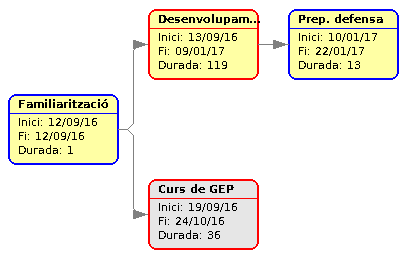
\includegraphics[width=\textwidth]{images/pert-global}
		\caption{PERT del projecte}
	\end{figure}

	\restoregeometry
	\newgeometry{bottom=1cm, top=1cm}
	\thispagestyle{empty}
	\begin{sidewaysfigure}
	%\begin{figure}[H]
		%\centering
		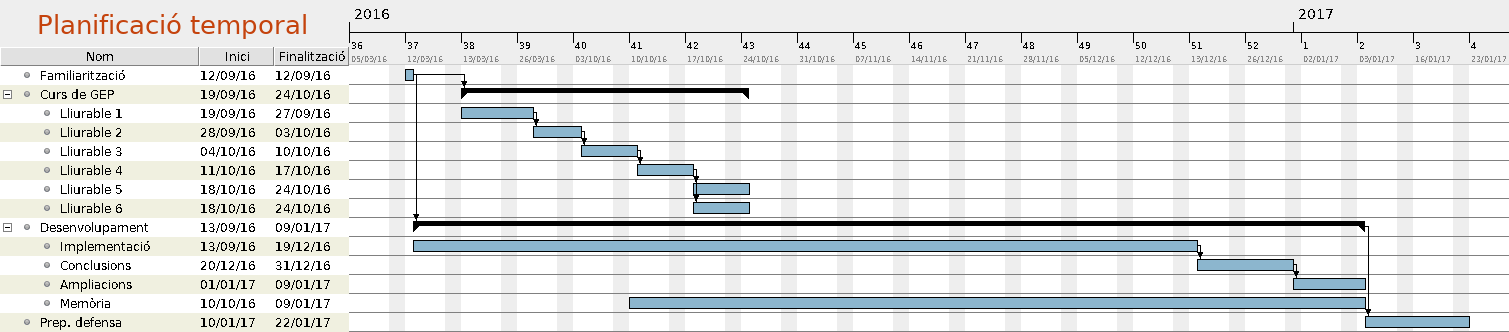
\includegraphics[width=\textheight]{images/gantt}
		\caption{Gantt del projecte}
	%\end{figure}
	\end{sidewaysfigure}


\restoregeometry
\newgeometry{bottom=4.5cm}

\section{Curs de GEP}
	\begin{figure}[H]
		\centering
		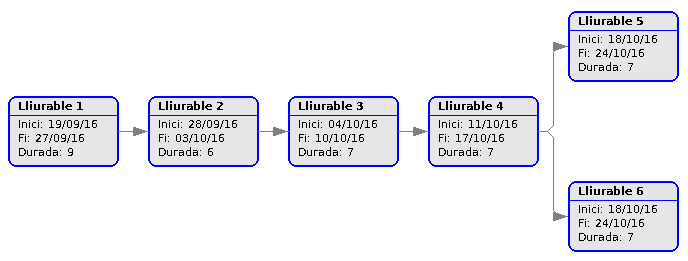
\includegraphics[width=\textwidth]{images/pert-gep}
		\caption{PERT - curs de GEP}
	\end{figure}

\section{Desenvolupament}
	\begin{figure}[H]
		\centering
		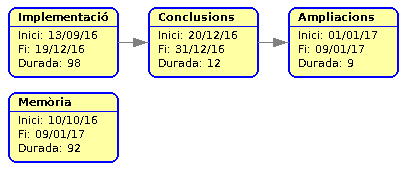
\includegraphics[width=\textwidth]{images/pert-dev}
		\caption{PERT - tasques desenvolupament}
	\end{figure}
\newpage

		\addtocontents{toc}{\setcounter{tocdepth}{2}}
	\end{appendices}

	\printbibliography[heading=bibintoc]
	\cleardoublepage\phantomsection\addcontentsline{toc}{chapter}{\listtablename}
	\listoftables
	\cleardoublepage\phantomsection\addcontentsline{toc}{chapter}{\listfigurename}
	\listoffigures
	
	

\end{document}
